\documentclass[a4paper]{article}

%%% Language and font encodings
%\usepackage[english]{babel}
\usepackage[utf8]{inputenc}
\usepackage{tabu}
\usepackage[T1]{fontenc}
\usepackage{enumitem}
\usepackage{amsmath}
\usepackage{xcolor}
\usepackage{amsfonts}
\usepackage{subfig}
\usepackage{wrapfig}
\usepackage{url}

%%% Sets page size and margins
\usepackage[a4paper,top=3cm,bottom=2cm,left=3cm,right=3cm,marginparwidth=1.75cm]{geometry}
\usepackage{mathbbol}
\usepackage{sidecap}

%%% Useful packages
\usepackage{amsmath}
\usepackage{graphicx}
\usepackage{fancyhdr}
\usepackage{makecell}

%\usepackage{subcaption}
%\usepackage[format=plain, indention=1cm]{caption}
\captionsetup[subfigure]{list=true, font=large, labelfont=bf, labelformat=brace, position=b, justification=centering}

%%% Define new commands
\renewcommand\theadalign{bc}
\renewcommand\theadfont{\bfseries}
\renewcommand\theadgape{\Gape[4pt]}
\renewcommand\cellgape{\Gape[4pt]}


%%% Title
\title{\textbf{Reinforcement Learning for Bomberman}
\\Final Project for the lecture:  \\Fundamentals of Machine Learning}
\author{Daniel Gonzalez, Matrikel Nr.: 3112012\\ Maria Regina Lily, Matrikel Nr.:  :)\\ Ferdinand Vanmaele, Matrikel Nr.: ;) \\ (Order alphebitcally, don't take it personal) }

\date{14.03.2019}

\begin{document}
\maketitle
\section{Abstract}
SOME TEXT - Look at the en in Conclusion for some useful links


\begin{figure}[h]

\includegraphics[scale=0.202]{images/img1}
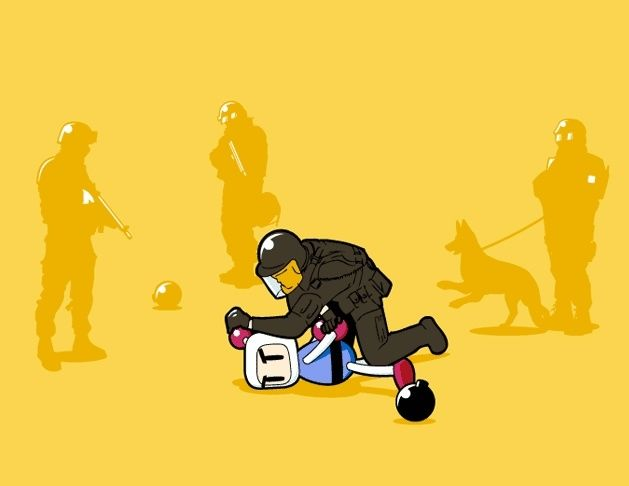
\includegraphics[scale=0.3]{images/img2}
\caption{he acts as a dement (left) he is often seen as a terrorist(right)}
\end{figure}
\section{Introduction}
[TODO: some text]

\section{Explaining the Framework}

\textbf{Features:}
\begin{itemize}

\item FOR STEP 1:
\begin{itemize} 
\item \textbf{1.)} Reward the best possible action to a coin, if it is reachable F(s,a)=1 ,  otherwise F(s,a)=0.    `BOMB' and `WAIT ' are always 0.
\end{itemize}

\item FOR STEP 1 \& 2:
\begin {itemize}
\item \textbf{1.)} \\  \textbf{DONE}  
\item  \textbf{2.)} Penalize if the action follows the agent to death (F,s)=1, F(s,a)=0. otherwise.  \\ \textbf{TO BE DONE: -> FERDINAND}
\item \textbf{3.)} Penalize if the action follows the agent into a ``save'':(Where the bomb won't at some point explode) position.  F(s,a)=1 otherwise F(s,a) = 0.  Bombs are always set to 0.
 \\  \textbf{TO BE DONE: -> DANIEL}  
 \item \textbf{4.)}  Reward the minimal distance that follows to safety if you are in a ``Danger zone'' (as defined in \textbf{3}.)  F(s,a)=1 otherwise F(s,a) = 0.
 If you are not in a ``Danger zone'' then F(s,a) =  0 for all actions.  For Bombs always set F(s,a) = 0.
  \\  \textbf{TO BE DONE: -> LILY}  
  \item \textbf{5.)} Penalize failure action F(s,a) = 1, otherwise F(s,a) = 0 .  
  BOMBS are always 0 and WAIT??
 \\  \textbf{TO BE DEFINED: WAIT ??}  
   \item \textbf{6.)} Reward when getting a coin F(s,a) = 1, otherwise F(s,a) = 0 .  
 \\  \textbf{DONE}  
 
    \item \textbf{7.)} Reward when destroying a block F(s,a) = 1, otherwise F(s,a) = 0 .  
 \\  \textbf{TO BE DONE: DANIEL}  
 
     \item \textbf{8.)} Reward (if there are no blocks anymore ? and no coins?)  the available movements F(s,a) = 1, otherwise F(s,a) = 0 .   Bombs = 0, WAIT =1 ? 
 \\  \textbf{TO BE DEFINE AND -> DANIEL}   
\end{itemize}



\end{itemize}

\subsection*{TD(0) learning}
[TODO: some text]
Probably not useful, but maybe useful as idea for loading images

\begin{minipage}{\columnwidth}
\makeatletter
\newcommand{\@captype}{figure}
\makeatother
\centering
\captionsetup[subfigure]{labelformat=empty}
\subfloat[\scriptsize Some text]{%

\includegraphics[scale=0.1]{images/img1}%
} \qquad \qquad%
\subfloat[\scriptsize Some text]{%

\includegraphics[scale=0.1]{images/img1} \quad

\includegraphics[scale=0.1]{images/img1}  }
\caption{Some text}
\label{fig-data-prep}
\end{minipage}


\subsection*{Gradient descent}
[TODO: some text]
Probably not useful, but maybe useful as idea for loading images
 \\ \\

\begin{minipage}{\columnwidth}
\makeatletter
\newcommand{\@captype}{figure}
\makeatother
\centering
\captionsetup[subfigure]{labelformat=empty}
\subfloat[ ]{%
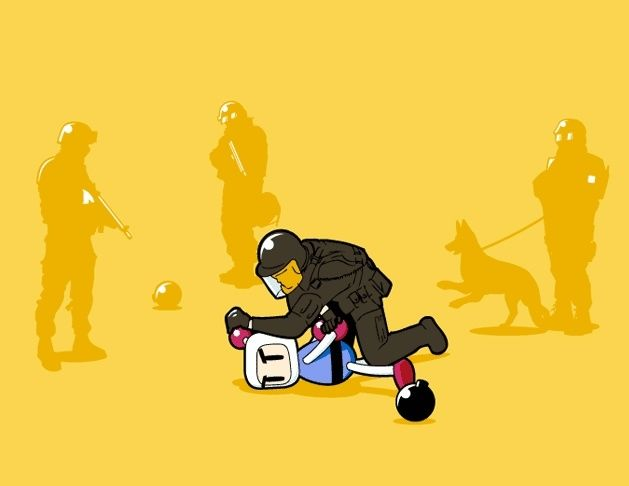
\includegraphics[scale=0.1]{images/img2}  \quad%  
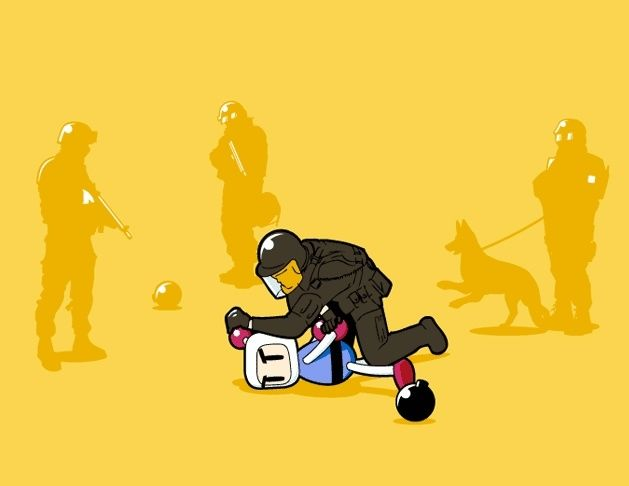
\includegraphics[scale=0.1]{images/img2}  \quad%  
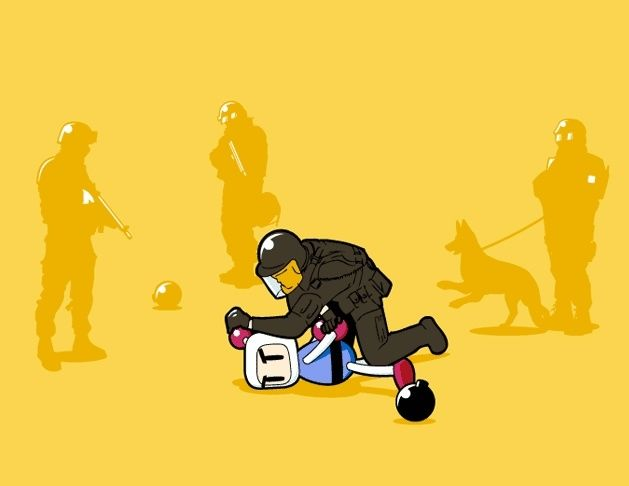
\includegraphics[scale=0.1]{images/img2}}  \qquad 
\subfloat{%
\vspace{1cm}
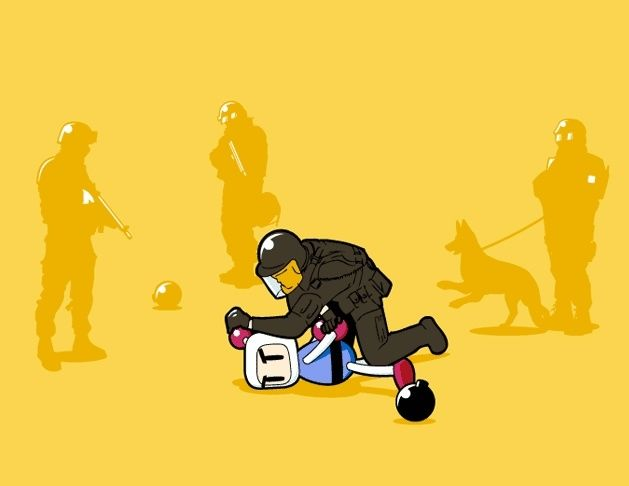
\includegraphics[scale=0.1]{images/img2}  \quad%  
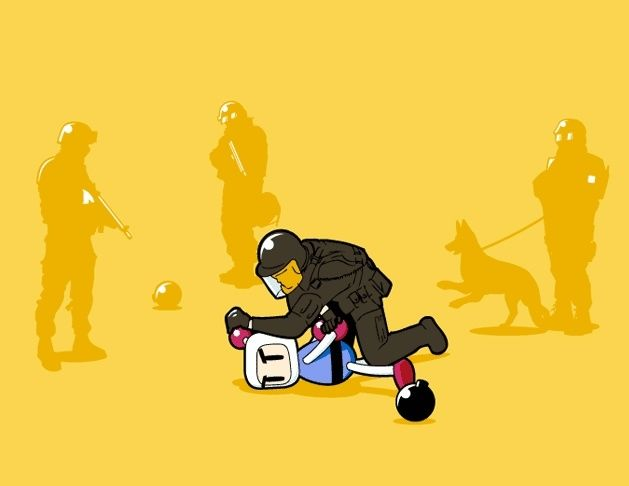
\includegraphics[scale=0.1]{images/img2}  \quad
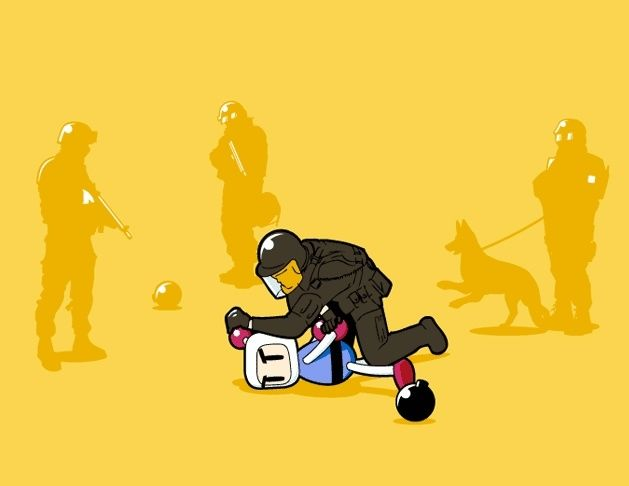
\includegraphics[scale=0.1]{images/img2} }
\caption{Some text}
\label{fig-canvas}
\end{minipage}
\newline \newline\newline 
\noindent Bla blah

\subsection*{Other sub chapter}
[SOME TEXT]. 

%\begin{minipage}{\columnwidth}
%\makeatletter
%\newcommand{\@captype}{figure}
%\makeatother
%\centering
%\captionsetup[subfigure]{labelformat=empty}
%\subfloat[0]{%
%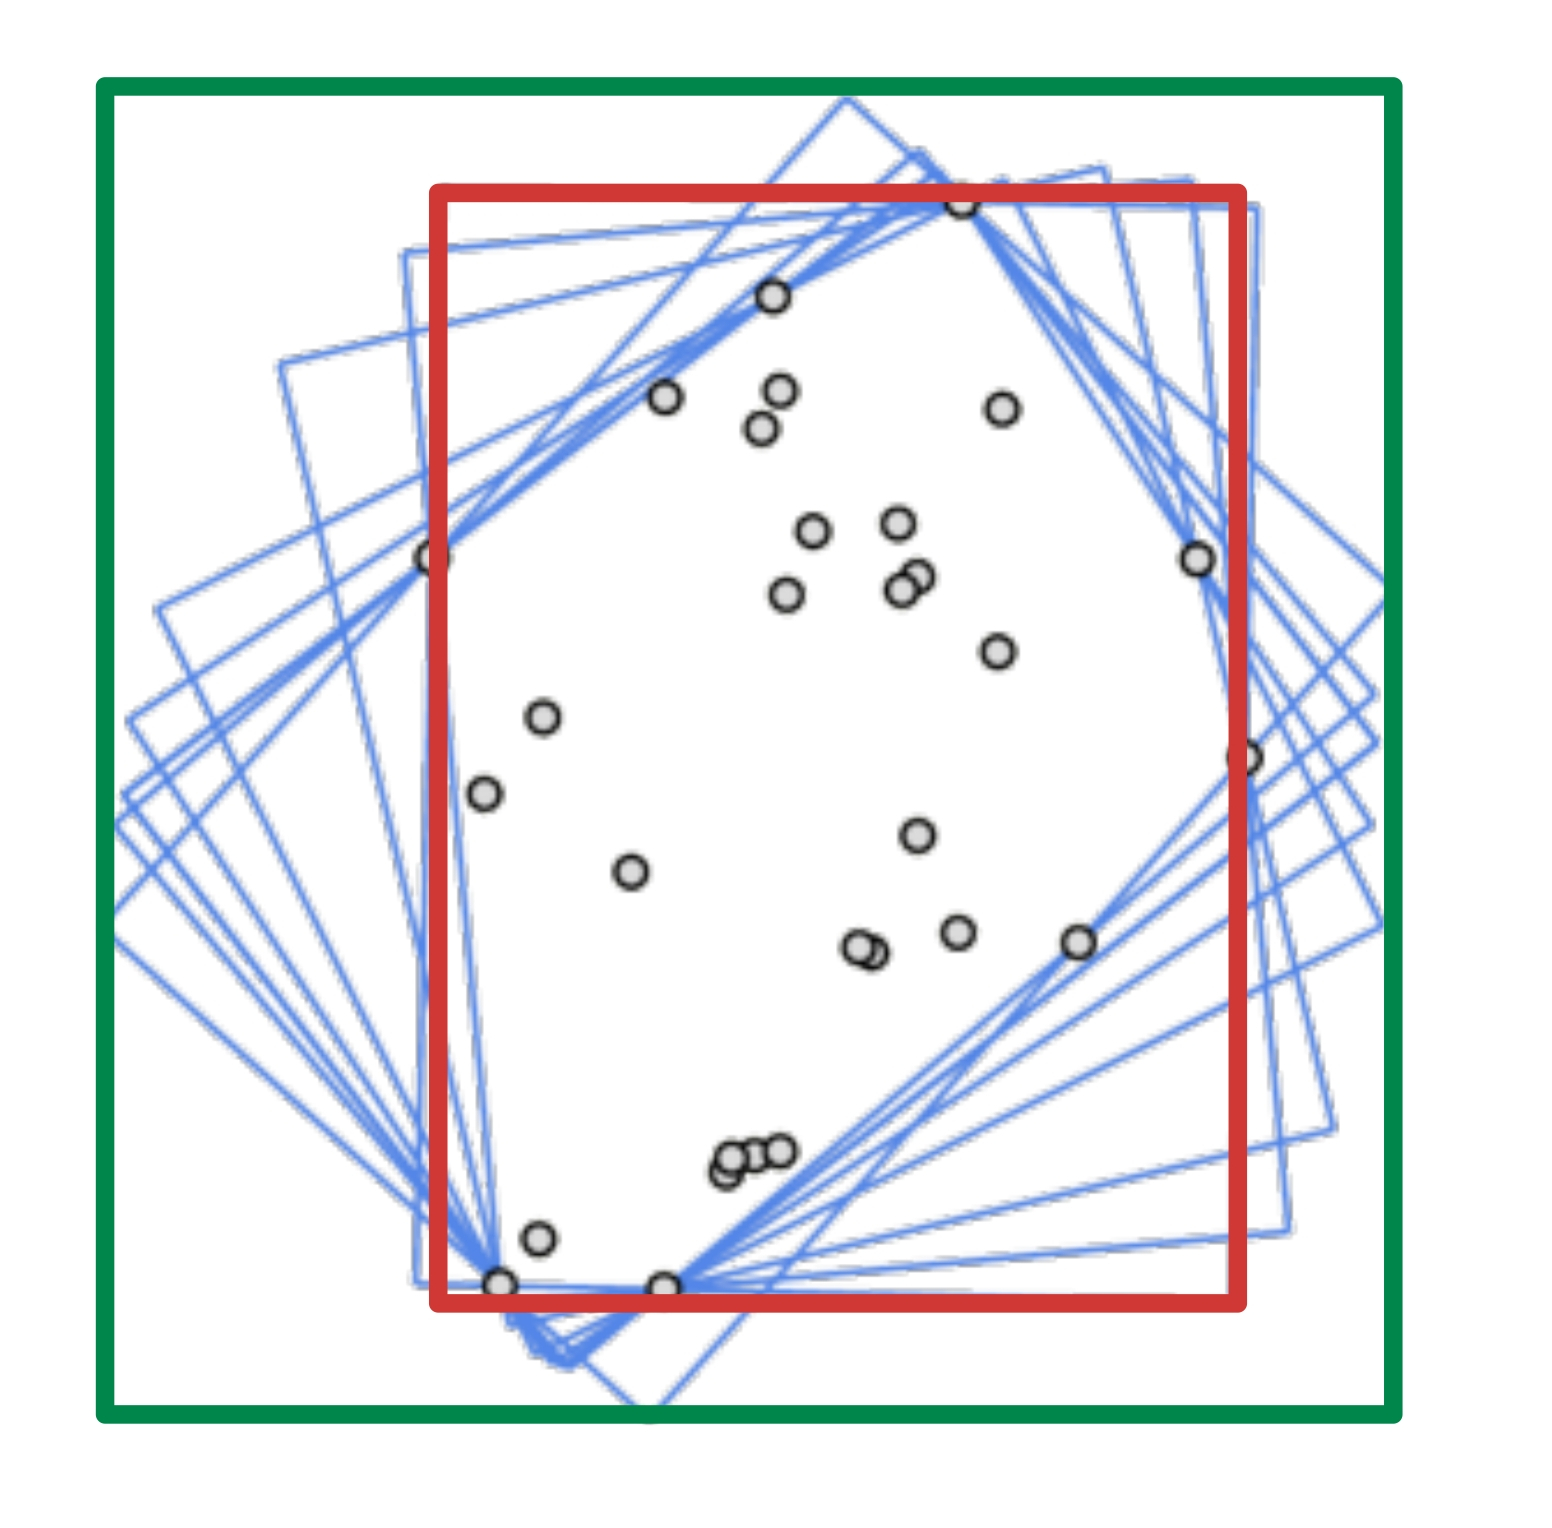
\includegraphics[scale=0.19]{images/ch_vs_bb}  }
%\caption{Green box represents the BB when applying some rotations, while the red box represents the BB of the convex hull.}
%\label{bb-ch}
%\end{minipage}

\begin{figure}[h]
\centering

\includegraphics[scale=0.15]{images/img1} 
\caption{some text}
\label{bb-ch}
\end{figure}

\newpage

\section{Related work}
[Some text]

\begin{wrapfigure}{l}{0.48\textwidth}
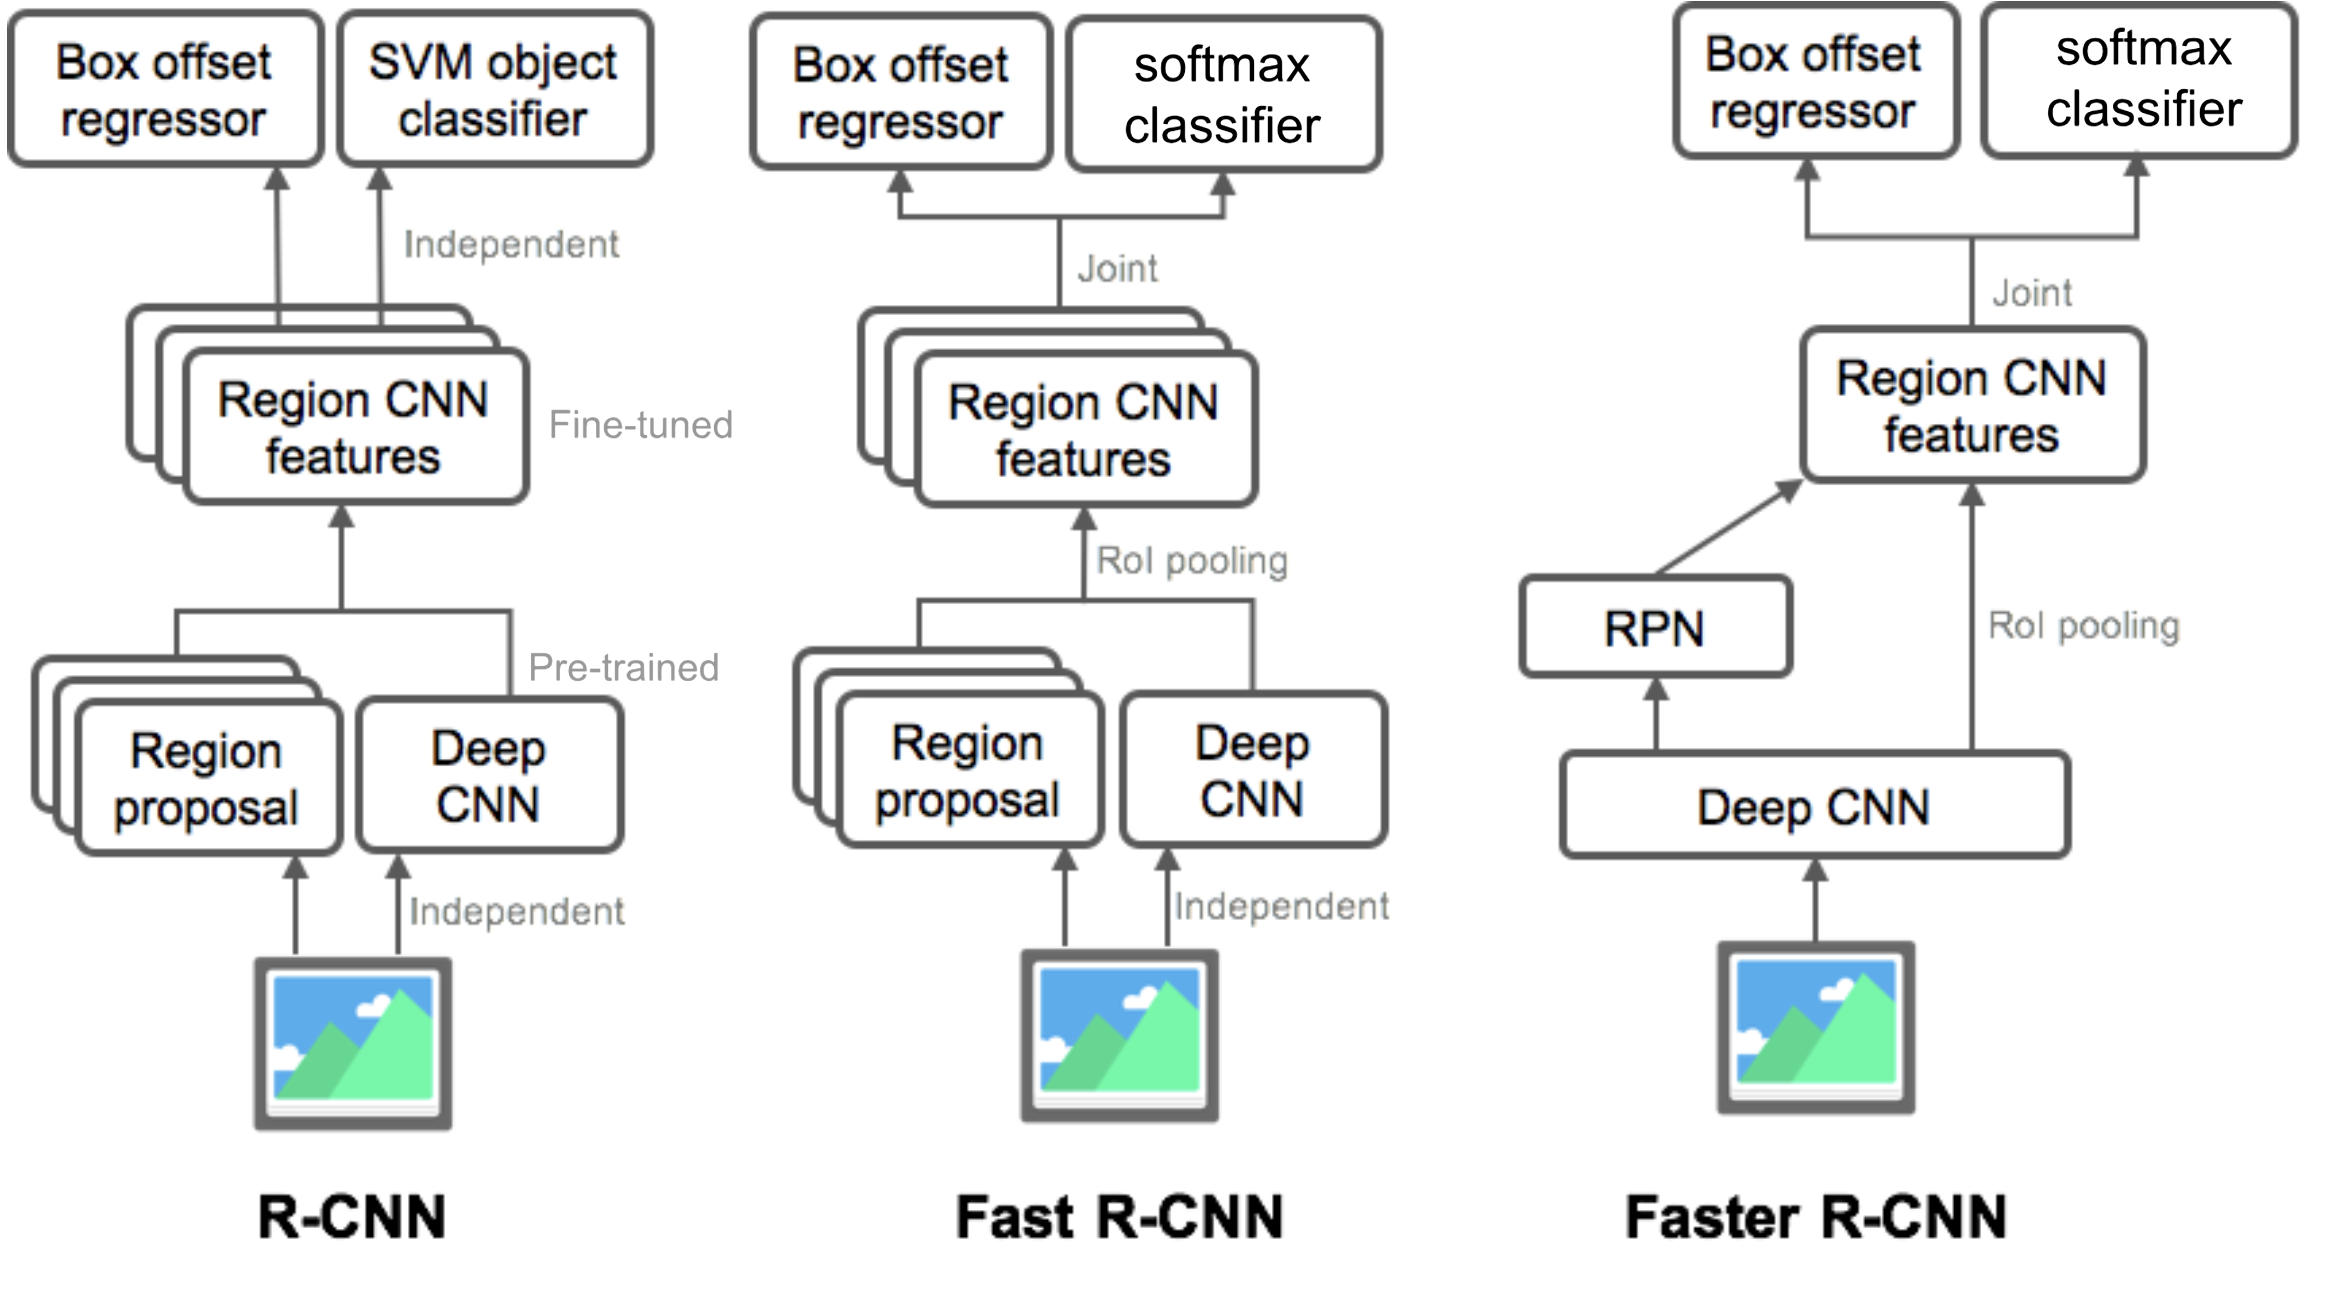
\includegraphics[scale=0.18]{images/FRCN_architecture}
\caption{SOME TEXT}
\label{fig:rcnn-architectures}
\end{wrapfigure} Some text \\ In 2015, \textbf{SOME TEXT}, \cite{DBLP:journals/corr/RenHG015}\textbf{)} (see Figure \ref{fig:rcnn-architectures}). 
\newline \newline \newline \newline \newline \newline \newline \newline\newline \newline\newline \newline\newline \newline\newline 
bla bla \\
\begin{wrapfigure}{h}{0.55\textwidth}

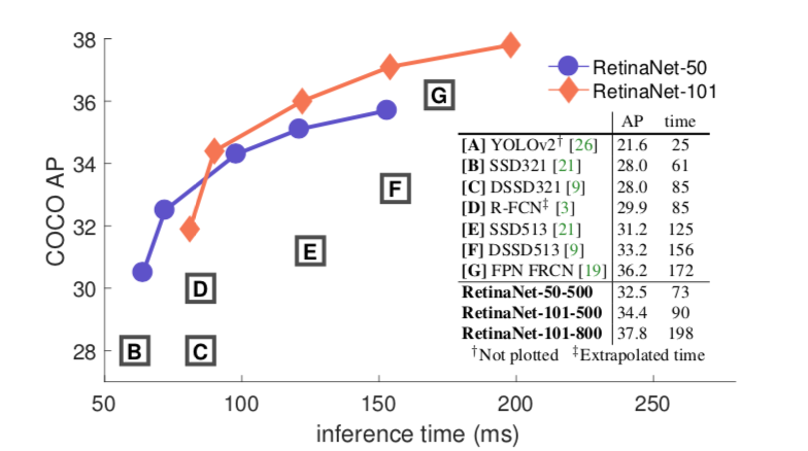
\includegraphics[scale=0.32]{images/retinanet}
\caption{some text}
\end{wrapfigure}
some citation examples 
 \cite{DBLP:journals/corr/abs-1708-02002}\cite{DBLP:journals/corr/LinDGHHB16} 

\section{See figures above (Strategy to also use space and have more variants for the text}
SOME TEXT
\newline 
\subsection*{The YOLO approach to object detection}
SOME TEXT

\begin{SCfigure}
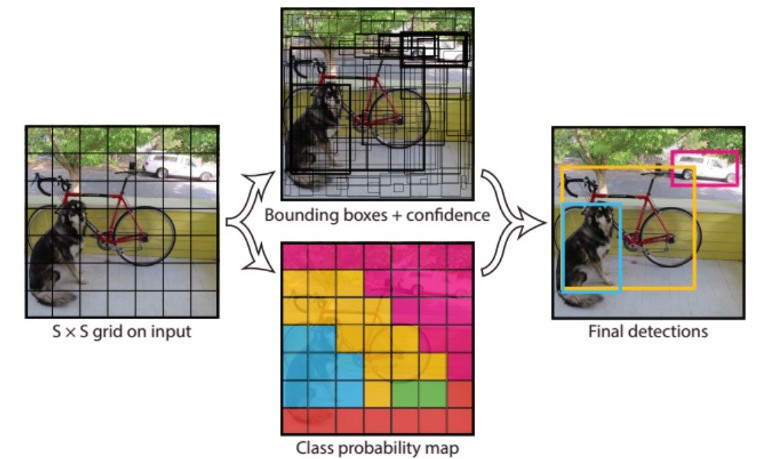
\includegraphics[scale=0.35]{images/yolo_model}\label{fig:yolomodel}
\caption{SOME TEXT.}
\end{SCfigure}


\subsubsection*{Anchor boxes}
SOME TEXT
\begin{SCfigure}
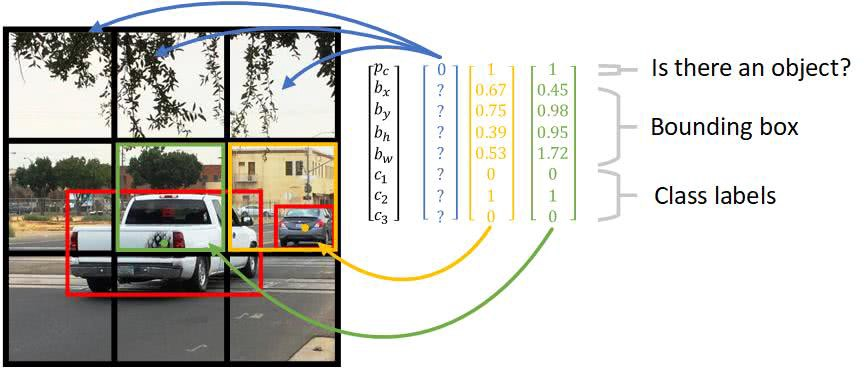
\includegraphics[scale=0.35]{images/yolo_mechanics}
\caption{SOME TEXT}
\label{fig:cell}
\end{SCfigure}



\subsubsection*{SUBSECTION}
SOME TEXT 

\subsubsection*{SUBSECTION}


\section{Feature extraction}
Some text

\section{Evaluation}
Some text

\section{Results:  some Table \& other way of loading images}
some text

\subsection*{some table }
\begin{table}[h]


\begin{tabular}{lllllr}
\hline
\multicolumn{5}{c}{Dataset situation} \\
\cline{1-2}
name    & description  & precision & recall & mAP \\
\hline
\textbf{1 - Simple}      & Paste cards on simple canvases    &  0.974  & 0.996 & \textbf{0.991} \\
          & \textit{random rotations, brightness, blurring}     & & & \\
\textbf{2 - Medium}      & Paste randomly scaled cards on simple canvases & 0.946 & 0.988 & \textbf{0.989} \\
          & \textit{random rotations, brightness, blurring}     & & & \\
\textbf{3 - Elaborate}       & Paste randomly scaled cards on textures & 0.937 & 0.978 & \textbf{0.971} \\
          & \textit{random rotations, brightness, blurring}     & & & \\
\textbf{4 - Hardest} & Paste randomly scaled cards on textures & 0.940 & 0.983 & \textbf{0.973} \\
          & \textit{random rotations, brightness, blurring, less zoom}     & & & \\
\hline


\end{tabular}
\caption{Precision and recall values have been calculated using a IOU threshold of 0.5. mAP values are based on averaged precision values over IOU thresholds of $[0.1, 0.2, \dots 0.8, 0.9] $  }
\label{tab:res}
\end{table}

\begin{figure}[h]

\begin{tabular}{ccc}

 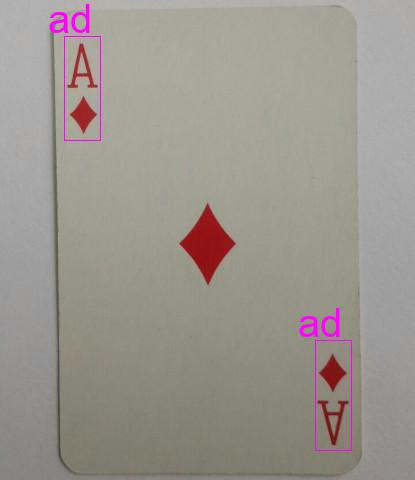
\includegraphics[height=44mm]{images/ad} &   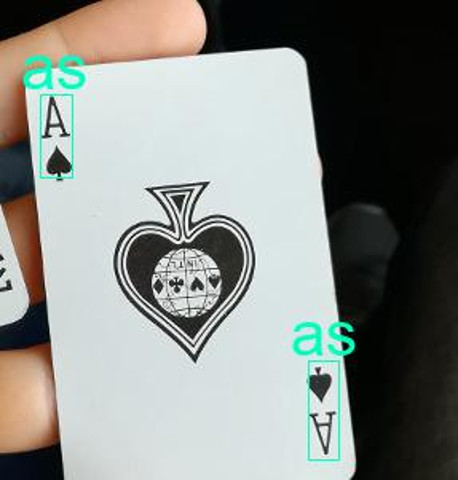
\includegraphics[height=44mm]{images/as} &   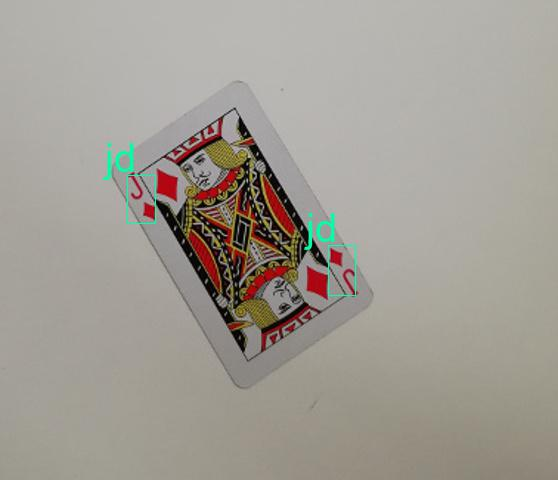
\includegraphics[height=44mm]{images/jd}\\
\makecell{\textbf{success:} classification: \\ \textbf{Ad:} 0.99995, \textbf{Ad:} 0.99997}  & \makecell{\textbf{success:}  classification \\ \textbf{As:} 0.99757, \textbf{As:} 0.99931} & \makecell{\textbf{success:}  classification \\ \textbf{Jd:} 0.99967, \textbf{Jd:} 0.99992}\\[6pt]

\end{tabular}
\caption{Successful cases of detection of images that are pretty representative of the training distribution}
\label{fig:testcases}
\end{figure}


\subsection*{Results of further work}
\subsubsection*{Transfer learning}

\subsubsection*{Webcam deployment}

\section{Discussion and Future Work  [Frank \& Daniel]}

\subsection*{Overview}

\subsubsection*{Training process}

\subsubsection*{Deployment on a webcam}


\subsection*{Future Work}



\section{Conclusion}
\url{https://github.com/mlteam-ws2018/RL_boom}.
SOME USEFUL LINKS (for the reportwriting):\newline
[for motivation]:  \url{https://www.youtube.com/watch?v=xMP-JqFQ_l4} \newline
[gd, policy, q-learning]:  \url{https://www.ias.informatik.tu-darmstadt.de/uploads/Theses/Sharma_BScThesis_2012.pdf} \newline
[gd, policy, q-learning]:  \url{https://repositorio-aberto.up.pt/bitstream/10216/91011/2/176444.pdf} \newline
\newpage
 \bibliographystyle{acm}

\bibliography{cite}
\end{document}
